\documentclass[hidelinks,12pt]{article}
\usepackage[left=0.25cm,top=1cm,right=0.25cm,bottom=1cm]{geometry}
%\usepackage[landscape]{geometry}
\textwidth = 20cm
\hoffset = -1cm
\usepackage[utf8]{inputenc}
\usepackage[spanish,es-tabla]{babel}
\usepackage[autostyle,spanish=mexican]{csquotes}
\usepackage[tbtags]{amsmath}
\usepackage{nccmath}
\usepackage{amsthm}
\usepackage{amssymb}
\usepackage{mathrsfs}
\usepackage{graphicx}
\usepackage{subfig}
\usepackage{standalone}
\usepackage[outdir=./Imagenes/]{epstopdf}
\usepackage{siunitx}
\usepackage{physics}
\usepackage{color}
\usepackage{float}
\usepackage{hyperref}
\usepackage{multicol}
%\usepackage{milista}
\usepackage{anyfontsize}
\usepackage{anysize}
%\usepackage{enumerate}
\usepackage[shortlabels]{enumitem}
\usepackage{capt-of}
\usepackage{bm}
\usepackage{relsize}
\usepackage{placeins}
\usepackage{empheq}
\usepackage{cancel}
\usepackage{wrapfig}
\usepackage[flushleft]{threeparttable}
\usepackage{makecell}
\usepackage{fancyhdr}
\usepackage{tikz}
\usepackage{bigints}
\usepackage{scalerel}
\usepackage{pgfplots}
\usepackage{pdflscape}
\pgfplotsset{compat=1.16}
\spanishdecimal{.}
\renewcommand{\baselinestretch}{1.5} 
\renewcommand\labelenumii{\theenumi.{\arabic{enumii}})}
\newcommand{\ptilde}[1]{\ensuremath{{#1}^{\prime}}}
\newcommand{\stilde}[1]{\ensuremath{{#1}^{\prime \prime}}}
\newcommand{\ttilde}[1]{\ensuremath{{#1}^{\prime \prime \prime}}}
\newcommand{\ntilde}[2]{\ensuremath{{#1}^{(#2)}}}

\newtheorem{defi}{{\it Definición}}[section]
\newtheorem{teo}{{\it Teorema}}[section]
\newtheorem{ejemplo}{{\it Ejemplo}}[section]
\newtheorem{propiedad}{{\it Propiedad}}[section]
\newtheorem{lema}{{\it Lema}}[section]
\newtheorem{cor}{Corolario}
\newtheorem{ejer}{Ejercicio}[section]

\newlist{milista}{enumerate}{2}
\setlist[milista,1]{label=\arabic*)}
\setlist[milista,2]{label=\arabic{milistai}.\arabic*)}
\newlength{\depthofsumsign}
\setlength{\depthofsumsign}{\depthof{$\sum$}}
\newcommand{\nsum}[1][1.4]{% only for \displaystyle
    \mathop{%
        \raisebox
            {-#1\depthofsumsign+1\depthofsumsign}
            {\scalebox
                {#1}
                {$\displaystyle\sum$}%
            }
    }
}
\def\scaleint#1{\vcenter{\hbox{\scaleto[3ex]{\displaystyle\int}{#1}}}}
\def\bs{\mkern-12mu}



\title{Esferas y la ecuación de Legendre \\ {\large Tema 4}\vspace{-3ex}}
\author{M. en C. Gustavo Contreras Mayén}
\date{ }

\pagestyle{fancy}
\fancyhf{}
\rhead{Curso MAF}
\lhead{\leftmark}
\rfoot{\thepage}
\setlength{\headheight}{16pt}%

\def\changemargin#1#2{\list{}{\rightmargin#2\leftmargin#1}\item[]}
\let\endchangemargin=\endlist 


\begin{document}
\maketitle
\fontsize{14}{14}\selectfont
\tableofcontents
\newpage

\section{Ecuación de Laplace.}

\subsection{Coordenadas esféricas.}

Para resolver la ecuación de Laplace:
\begin{align*}
\laplacian{\Psi} = 0
\end{align*}
en un sistema coordenado esférico $(r, \theta, \varphi)$, hacemos el cambio entre el sistema cartesiano y el esférico, teniendo entonces:
\begin{align}
\begin{aligned}[b]
\dfrac{1}{r^{2}} \pdv{r} \left( r^{2} \pdv{\Psi}{r} \right) &+ \dfrac{1}{r^{2} \, \sin \theta} \bigg[ \pdv{\theta} \left( \sin \theta \pdv{\Psi}{\theta} \right) + \dfrac{1}{\sin \theta} \, \pdv[2]{\Psi}{\varphi} \bigg] = 0
\end{aligned}
\label{eq:ecuacion_22_15}
\end{align}

\subsection{Separación de variables.}

Para ocupar la técnica de separación de variables, proponemos una solución del tipo:
\begin{align*}
\Psi(r, \theta, \varphi) = R(r) \, \Theta \, (\theta) \, \Phi(\varphi)
\end{align*}
Que sustituimos en la ec (\ref{eq:ecuacion_22_15}), y cuyo procedimiento ya sabemos realizar, así tenemos que:
\begin{align*}
\Theta \Phi \dfrac{1}{r^{2}} \, \dv{r} \left( r^{2} \dv{R}{r} \right) + \dfrac{R}{r^{2}} \bigg[ \dfrac{\Phi}{\sin \theta} \, \dv{\theta} \left( \sin \theta \dv{\Theta}{\theta} \right) + \dfrac{\Theta}{\sin^{2} \theta} \, \dv[2]{\Phi}{\varphi} \bigg] = 0
\end{align*}
donde encontramos que cada derivada se realiza sobre cada una de las variables. Al dividir entre $R \, \Theta \, \Phi$ y luego multiplicar por $r^{2}$, llegamos a:
\begin{align*}
\dfrac{1}{R} \, \dv{r} \left( r^{2} \dv{R}{r} \right) + \bigg[ \dfrac{1}{\Theta \sin \theta} \, \dv{\theta} \left( \sin \theta \dv{\Theta}{\theta} \right) + \dfrac{1}{\Phi \sin^{2} \theta} \, \dv[2]{\Phi}{\varphi} \bigg] = 0
\end{align*}
ya que cada uno de los términos es función de variables independientes, por tanto deben de ser una constante, y las dos constantes deben de sumar cero. Así obtenemos:
\begin{align*}
\dfrac{1}{R} \, \dv{r} \left( r^{2} \dv{R}{r} \right) &= \alpha \\[0.5em]
\dfrac{1}{\Theta \sin \theta} \, \dv{\theta} \left( \sin \theta \dv{\Theta}{\theta} \right) + \dfrac{1}{\Phi \sin^{2} \theta} \, \dv[2]{\Phi}{\varphi} &= - \alpha
\end{align*}
La segunda ecuación debe de separarse nuevamente, agregamos $\alpha$ en ambos lados de la expresión y multiplicamos por $\sin^{2} \theta$, llegando a:
\begin{align*}
\dfrac{\sin \theta}{\Theta} \, \dv{\theta} \left( \sin \theta \dv{\Theta}{\theta} \right) + \alpha \, \sin^{2} \theta +  \dfrac{1}{\Phi} \, \dv[2]{\Psi}{\varphi} = 0
\end{align*}
que siguiendo el mismo razonamiento, tendremos una segunda constante de separación:
\begin{align*}
\dfrac{\sin \theta}{\Theta} \, \dv{\theta} \left( \sin \theta \dv{\Theta}{\theta} \right) &= \beta \\[0.5em]
\dfrac{1}{\Phi} \, \dv[2]{\Phi}{\varphi} = - \beta
\end{align*}
De modo que hemos recuperado tres EDO2H, cada una de una sola variable:
\begin{align}
\dfrac{1}{r^{2}} \, \dv{r} \left( r^{2} \dv{R}{r} \right) - \dfrac{\alpha}{r^{2}} \, R &= 0 \label{eq:ecuacion_22_17a} \\[0.5em]
\dfrac{1}{\sin \theta} \, \dv{\theta} \left( \sin \theta \dv{\Theta}{\theta} \right) + \left( \alpha - \dfrac{\beta}{\sin^{2} \theta} \right) \, \Theta &= 0 \label{eq:ecuacion_22_17b} \\[0.5em]
\dv[2]{\Phi}{\varphi} + \beta \, \Phi &= 0 \label{eq:ecuacion_22_17c}
\end{align}
La ec. (\ref{eq:ecuacion_22_17a}) se conoce como \textbf{ecuación radial}, mientras que la ec. (\ref{eq:ecuacion_22_17b}) es la \textbf{ecuación polar}, la tercera ec. (\ref{eq:ecuacion_22_17c}) es la \textbf{ecuación azimutal}.

\subsection{Simetría azimutal.}

Consideramos el caso donde $\Phi$ es la función constante, esto corresponde a problemas con una \emph{simetría azimutal}, es decir, problemas para los cuales está claro a priori que el potencial es independiente del ángulo azimutal $\varphi$. En tales situaciones, la ec. \ref{eq:ecuacion_22_17c}) implica que $\beta = 0$ porque $\Phi$ es una constante (distinta de cero). Las variables independientes se reducen a dos y, con \break \hfill $\psi (r, \theta) = R (r) \, \Theta (\theta)$, las EDO2H restantes se simplifican:
\begin{align}
\begin{aligned}
\dfrac{1}{r^{2}} \dv{r} \left( r^{2} \dv{R}{r} \right) - \dfrac{\alpha}{r^{2}} \, R &= 0 \\[0.5em]
\dfrac{1}{\sin \theta} \dv{\theta} \left( \sin \theta \dv{\Theta}{\theta} \right) + \alpha \, \Theta &= 0
\end{aligned}
\label{eq:ecuacion_26_02}
\end{align}

\subsection{Resolviendo las EDO2H.}

De manera inicial nos enfocamos en la ecuación polar. La presencia en el denominador del término $\sin \theta \dd{\theta}$ (que es el diferencial de $\cos \theta)$ sugiere el cambio de variable de $\theta$ a $u \equiv \cos \theta$. Para cualquier función $f (\theta)$, con la regla de la cadena se tiene:
\begin{align*}
\dv{f}{u} = \dv{f}{\theta} \dv{\theta}{u} = \dv{f}{\theta} \dfrac{1}{\dv*{u}{\theta}} = - \dfrac{1}{\sin \theta} \dv{f}{\theta}
\end{align*}
De manera equivalente:
\begin{align}
\dv{f}{\theta} = - \sin \theta \dv{f}{u}
\label{eq:ecuacion_26_03}
\end{align}
Esto nos permite convertir la derivada de una función con respecto a $u$, en la derivada de la misma función con respecto a $\theta$.
\par
Proponemos una función $P(u)$ tal que:
\begin{align*}
P(u) = \Theta(\theta)
\end{align*}
Usamos la regla de la cadena mostrada, sustituyendo en la ecuación polar y escribiendo $\sin^{2} \theta = 1 - u^{2}$, la EDO pasa a ser:
\begin{align*}
- \dfrac{1}{\sin \theta} \dv{\theta} \bigg[ (1 - u^{2}) \dv{P}{u} \bigg] + \alpha \, P = 0
\end{align*}
El término en el corchete es función de $u$. Ocupando la ec. (\ref{eq:ecuacion_26_03}), podemos convertir la derivada en $\theta$ en una derivada en $u$, para así obtener:
\begin{align}
\dv{u} \bigg[ (1 - u^{2}) \dv{P}{u} \bigg] + \alpha P = 0
\label{eq:ecuacion_26_04}
\end{align}
Que se puede escribir como:
\begin{align}
(1 - u^{2}) \, \dv[2]{P}{u} - 2 \, u \, \dv{P}{u} + \alpha \, P = 0
\label{eq:ecuacion_26_05}
\end{align}
De manera equivalente:
\begin{align}
\dv[2]{P}{u} - \dfrac{2 \, u}{1 - u^{2}} \, \dv{P}{u} + \dfrac{\alpha}{(1 - u^{2})} \, P = 0
\label{eq:ecuacion_26_06}
\end{align}
A esta ecuación se le conoce como la \textbf{ecuación diferencial de Legendre}.
\par
Las soluciones a la ecuación de Legendre son los polinomios de Legendre de orden $n$: $P_{n} (x)$, y se detallan en las notas de trabajo, por lo que aquí haremos uso de las mismas y de sus propiedades.

\subsection{Ecuación radial.}

En la solución de la ecuación angular, se determina que $\alpha = k (k + 1)$, de esta manera la ecuación radial se escribe como:
\begin{align}
r^{2} \dv[2]{R}{r} + 2 R \dv{R}{r} - k(k + 1) R = 0
\label{eq:ecuacion_26_28}
\end{align}
Como $p_{2} (0) = 0$, se considera una solución a la ecuación radial de la forma:
\begin{align*}
R(r) = r^{s} \nsum_{n=0}^{\infty} b_{n} \, r^{n}
\end{align*}
es decir, hacemos un desarrollo con el método de Frobenius. La solución general a la ecuación radial es entonces:
\begin{align*}
R_{k}(r) \equiv A_{k} \, r^{k} + \dfrac{B_{k}}{r^{k+1}} \hspace{0.3cm} k = 0, 1, 2, \ldots
\end{align*}
con $A_{k}$ y $B_{k}$ coeficientes por determinar.

\section{Solución completa.}

Para encontrar la solución general a la ecuación de Laplace en coordenadas esféricas con una simetría azimutal, multiplicamos la solución radial y angular (dada por los polinomios de Legendre) para cada $k$ y se suma en todos los valores posibles de $k$:
\begin{align}
\psi(r, \theta) = \nsum_{k=0}^{\infty} \left( A_{k} \, r^{k} + \dfrac{B_{k}}{r^{k+1}} \right) \, P_{k} (\cos \theta)
\label{eq:ecuacion_26_29}
\end{align}
donde se ha cambiado $\cos \theta$ por $u$.

\section{Esferas y temperaturas.}

Dos hemisferios sólidos conductores de calor de radio $a$, separados por un pequeño espacio aislante, forman una esfera. Las dos mitades de la esfera están en contacto en el exterior, con dos baños de calor (infinitos) a temperaturas $T_{0}$ y $-T_{0} $, ver la figura (\ref{fig:figura_esfera_01}):
\begin{figure}[H]
    \centering
    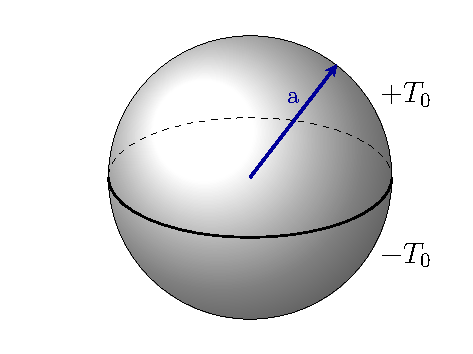
\includegraphics[scale=0.95]{Imagenes/Ejemplo_Esfera_01.eps}
    \caption{Dos hemisferios a distintas temperaturas.}
    \label{fig:figura_esfera_01}
\end{figure}

\textbf{Queremos encontrar la distribución de temperatura $T (r, \theta, \varphi)$ en puntos dentro de la esfera.}
\par
Ya tenemos una expresión que nos permitirá resolver el ejercicio, considerando algunos puntos importantes. En este ejercicio se muestra que es muy importante tomar en cuenta las características que presenta un problema: geometría involucrada, ecuación que modela el fenómeno, técnica de solución a la ecuación, etc.

\subsection{Identificando puntos importantes.}

Elegimos un sistema de coordenadas esféricas en el que el origen coincide con el centro de la esfera y el eje polar es perpendicular al plano ecuatorial. Suponemos que el hemisferio con temperatura $T_{0}$ es el hemisferio norte, el hemisferio sur está a la temperatura $-T_{0}$.
\par
Dado que el problema tiene simetría azimutal, $T$ es independiente de $\varphi$, y podemos escribir inmediatamente la solución general con simetría azimutal de la ecuación Laplace en coordenadas esféricas:
\begin{align*}
\psi (r, \theta) = \nsum_{k=0}^{\infty} \left( A_{k} \, r^{k} + \dfrac{B_{k}}{r^{k+1}} \right) \, P_{k} (\cos \theta)
\end{align*}
Sin embargo, dado que el origen $r = 0$ está en la región de interés, debemos excluir todos los potencias negativas de $r$.  Esto se logra haciendo que $B_{k} = 0$. Así, tenemos:
\begin{align}
T (r, \theta) = \nsum_{n=0}^{\infty} A_{n} \, r^{n} \, P_{n} (\cos \theta)
\label{eq:ecuacion_26_50}
\end{align}
Quedando pendiente el cálculo de los coeficientes $A_{n}$. Para resolver esta parte, revisemos que:
\begin{align*}
T (a, \theta) = \begin{cases}
T_{0} & \mbox{ si } 0 \leq \theta < \dfrac{\pi}{2} \\[1em]
-T_{0} & \mbox{ si } \dfrac{\pi}{2} < \theta \leq \pi
\end{cases}
\end{align*}
En términos de $u = \cos \theta$, queda expresado por:
\begin{align}
T (a, u) = \begin{cases}
-T_{0} & \mbox{ si } -1 \leq u < 0 \\[1em]
T_{0} & \mbox{ si } 0 < u \leq 1
\end{cases} = \nsum_{n=0}^{\infty} A_{n} \, a_{n} \, P_{n} (u)
\label{eq:ecuacion_26_51}
\end{align}
que, excepto por el uso de $u$ en lugar de $x$, es completamente equivalente a la expansión del ejemplo que se encuentra en las notas de trabajo, donde encontramos que los coeficientes pares están ausentes y:
\begin{align*}
c_{2k+1} \equiv A_{2k+1} \, a^{2k+1} = \dfrac{(-1)^{k} (4 \, k + 3)(2 \, k)!}{2^{2k+1} \, k! \, (k+1)!} \, T_{0}
\end{align*}
Despejando $A_{2k+1}$ de la ecuación anterior, para utilizarlo dentro de la ec. (\ref{eq:ecuacion_26_50}) nos lleva a la solución, que \emph{determina la temperatura en puntos interiores de la esfera}:
\begin{align}
T (r, \theta) = T_{0} \, \nsum_{k=0}^{\infty} \dfrac{(-1)^{k} (4 \, k {+} 3)(2 \, k)!}{2^{2k+1} \, k! \, (k {+} 1)!} \, \left( \dfrac{r}{a} \right)^{2k+1} \, P_{2k+1} (\cos \theta)
\label{eq:ecuacion_26_52}
\end{align}
donde se ha sustituido $\cos \theta$ por $u$.

\section{Esferas y potenciales.}

Considere dos hemisferios eléctricamente conductores de radio $a$ separados por un pequeño espacio aislante en el ecuador. El hemisferio superior se mantiene en el potencial $V_{0}$ y el inferior en $-V_{0}$, tal como se muestra en la figura (\ref{fig_figura_esfera_03}).
\par
\textbf{Queremos encontrar el potencial en puntos fuera de la esfera resultante}.
\begin{figure}[H]
    \centering
    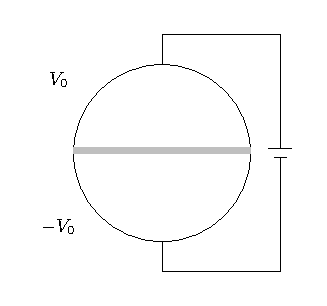
\includegraphics[scale=1.3]{Imagenes/Ejemplo_Esfera_03.eps}
    \caption{Dos hemisferios conductores cada uno con un potencial. El hemisferio superior tiene un rango para el ángulo polar $0 \leq \theta < \pi/2$ o $0 < \cos \theta \leq 1$, mientras que el hemisferio inferior tiene el rango $\pi/2 < \theta \leq \pi $ o $-1 \leq \cos \theta < 0$.}
    \label{fig_figura_esfera_03}
\end{figure}

Dado que el potencial debe anularse en el infinito, esperamos que el primer término en la ecuación (\ref{eq:ecuacion_26_29}) esté ausente, es decir, debe de ocurrir que $A_{k} = 0$. Para encontrar $B_{k}$, sustituimos $a$ por $r$ en la ec. (\ref{eq:ecuacion_26_29}), y sea $\cos \theta \equiv u$. Entonces:
\begin{align*}
\psi (a, u) = \nsum_{k=0}^{\infty} \underbrace{\dfrac{B_{k}}{a^{k+1}}}_{\mbox{\large $\equiv c_{k}$}} \, P_{k} (u)
\end{align*}
donde:
\begin{align*}
\psi (a, u) = \begin{cases}
- V_{0} & \mbox{ si } -1 \leq u < 0 \\[1em]
+ V_{0} & \mbox{ si } 0 < u \leq 1
\end{cases}
\end{align*}
El cálculo de los coeficientes es idéntico al del ejemplo de las notas de trabajo. Por lo tanto, $c_{k} = 0$ para $k$ par y:
\begin{align*}
c_{2m+1} = \dfrac{B_{2m+1}}{a^{2m+2}} = (-1)^{m} \, \dfrac{(4 m + 3)(2 m)!}{2^{2m+1} (m + 1)! m!} \, V_{0}
\end{align*}
Que despejando para los coeficientes $B_{2m+1}$:
\begin{align*}
B_{2m+1} = \dfrac{(-1)^{m} \, (4 m + 3)(2 m)!}{2^{2m+1} m! (m + 1)!} \, a^{2m+2} \, V_{0}
\end{align*}
Una vez que se calcularon los coeficientes, el potencial queda dado por:
\begin{align}
\psi (r, \theta) = V_{0} \nsum_{m=0}^{\infty} (-1)^{m} \, \dfrac{(4 m + 3)(2 m)!}{2^{2m+1} m! (m + 1)!} \, \left( \dfrac{a}{r} \right)^{2m+2} \, P_{2m+1} (\cos \theta)
\label{eq:ecuacion:26_53}
\end{align}

% \section{Ejercicio esfera aterrizada.}

% Veamos otro ejemplo de la solución de la ecuación de Laplace en coordenadas esféricas, consideremos una esfera conductora neutra puesta a tierra de radio $a$ colocada en un campo eléctrico originalmente uniforme $E_{0}$ que se supone que tiene una extensión infinita, como se muestra en la figura (\ref{fig:figura_esfera_aterrizada})).
% \begin{figure}[H]
%     \centering
%     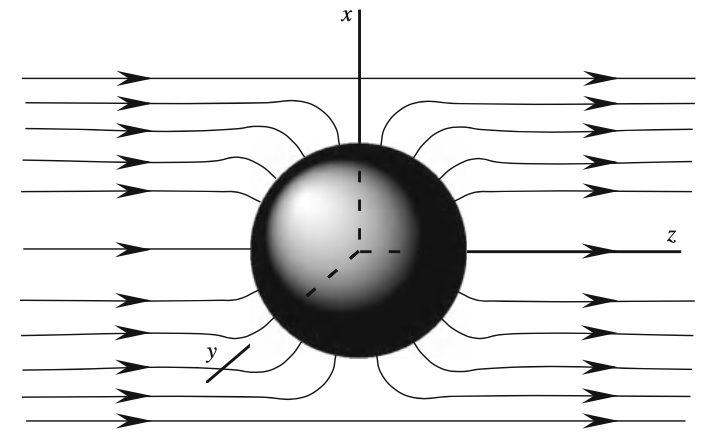
\includegraphics[scale=0.4]{Imagenes/Esfera_Compo_Electrico.png}
%     \caption{El campo eléctrico en la vecindad de una esfera colocada en un campo uniforme externo cambiará, pero el campo alejado de la esfera permanecerá casi uniforme.}
%     \label{fig:figura_esfera_aterrizada}
% \end{figure}

% \textbf{Queremos encontrar el potencial electrostático en todas partes fuera de la esfera}.
% \par
% Eligiendo que el campo esté en la dirección $z$ positiva y colocando el centro de la esfera en el origen, tendremos un problema que presenta simetría azimutal. Por lo tanto, la solución general viene dada por la ec. (\ref{eq:ecuacion_26_29}). Los límites por fuera de la esfera consisten en la esfera misma así como en el infinito. El campo eléctrico en el infinito es el campo uniforme original, porque el campo debido a las cargas inducidas en la esfera desaparece en el infinito. El potencial de este campo (en el infinito) se puede deducir de:
% \begin{align*}
% \vb{E} &= E_{0} \, \vu{e}_{z} = - \grad{\Phi} \\[0.5em]
% \Rightarrow \hspace{0.2cm} E_{0} &= - \pdv{\Phi}{z}, \hspace{1cm} \pdv{\Phi}{x} = \pdv{\Phi}{y} = 0
% \end{align*}
% Por lo tanto, el potencial en el infinito es independiente de $x$ e $y$, y se puede escribir como:
% \begin{align*}
% \Phi (r, \theta) &= - E_{0} \, z = \\[0.5em]
% &= - E_{0} \, r \, \cos \theta = \\[0.5em]
% &= - E_{0} \, r \, P_{1} (\cos \theta) \hspace{1cm} \mbox{para } r \to \infty
% \end{align*}
% Por lo tanto, el potencial en el infinito es independiente de $x$ e $y$, y se puede escribir como:

\end{document}